\chapter{11.Mathematischer Nachschlag}
Aus mathematischer Sicht sind einige Fragen offen geblieben, etwa:

\newcommand{\D} {
\mathcal{D}
}

\section{Verallgemeinerte Funktionen und Abbleitungen}
Wie differenziert man unstetige Funktionen?

Sei $\D := C_0^\infty(\R^d)$ die Menge (auch ein Vektorraum) der beliebig oft differenzierbaren Funktionen auf $\R^d$ mit beschränktem Träger. Etwa:

\begin{center}
    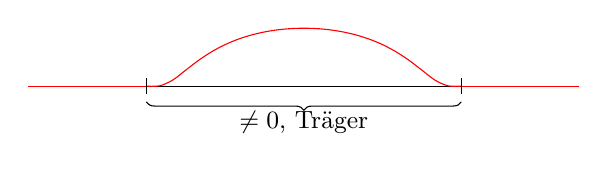
\begin{tikzpicture}
        \draw (-3,0) -- (3,0);
        \draw[scale=2,domain=-0.999:0.999,smooth,variable=\x,red] plot ({\x},{e^(-(1 - abs(\x)^2 )^(-1)});
        \draw[red] (-3.5,0) -- (-0.999*2,0);
        \draw[red] (3.5,0) -- (0.999*2,0);
        \draw (0.999*2,-0.1) -- (0.999*2,0.1);
        \draw (-0.999*2,-0.1) -- (-0.999*2,0.1);
        \draw[decorate,decoration={brace,amplitude=3pt,mirror}] (-2,-0.2) -- node[below] {\small $\neq0$, Träger} (2,-0.2);
    \end{tikzpicture}
\end{center}

Diese Funktion ist:

\[\varphi(x)=g(1- \abs{x}^2)\]

wobei

\[g(t) := \begin{cases}
    e^{\frac{-1}{t}} & ,t>0\\
    0 & ,t\leq 0
\end{cases}\]

Dieses Funktioniert auch im $\R^d$

\def\centerx{2}
\def\centery{-1}

\begin{center}
    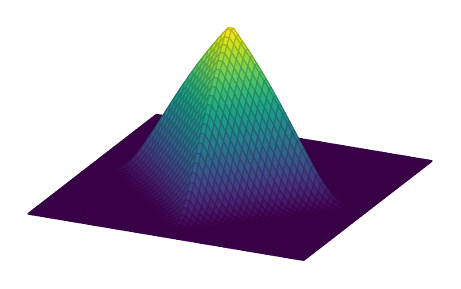
\begin{tikzpicture}[        declare function={
        func(\x) = (\x>0) * e^(-(\x)^(-1)) +
                   (\x<=0) * 0;
      }]

        \pgfplotsset{
            colormap name=viridis,
        }
            \begin{axis}[hide axis,scale=0.75,name=plot1,samples=10]
                \addplot3[surf,domain=-1:1,domain y=-1:1,samples=60]
                    {func(1 - abs(x) - abs(y)))};
                \end{axis}
    \end{tikzpicture}
\end{center}

ist $C_0^\infty(\R^d)$ und hat kompakten Träger.

Sei nun $L^1_{loc}(\R^d)$ die Menge aller Funktionen auf $\R^d$ mit kompaktem Träger für die:

\[\int_K \abs{f(x)} dx < \infty\]

für alle abgeschlossenen und beschränkten Mengen $K \subset \R^d$ gilt.

\begin{center}
    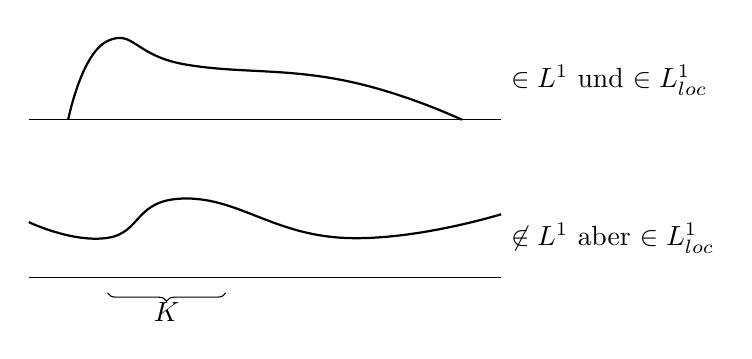
\begin{tikzpicture}
        \draw (-3,0) -- (3,0);
        \draw[thick] plot [smooth, tension = 0.8] coordinates {(-2.5,0) (-2,1)  (-1,0.7) (1,0.5) (2.5,0)};
        \draw (3,0.5) node[right] {$\in L^1$ und $\in L^1_{loc}$};
        \draw (-3,-2) -- (3,-2);
        \draw[thick] plot [smooth, tension = 0.8] coordinates {(-3,-1.3) (-2,-1.5) (-1,-1) (1,-1.5) (3,-1.2) };
        \draw (3,-1.5) node[right] {$\not \in L^1$ aber $\in L^1_{loc}$}; 
        \draw[decorate,decoration={brace,amplitude=3pt,mirror}] (-2,-2.2) -- node[below] {$K$} (-0.5,-2.2);
    \end{tikzpicture}
\end{center}

Die Zweite Funktion ist nicht in $L^1$ da ihr Gesamtintegral nicht endlich ist jedoch ist das Integral über jede endlich Menge endlich, sie hat also keine Pole, somit sie in $L^1_{loc}$.

Für jede Funktion $f \in L^1_{loc}(\R^d)$ bildet 
\begin{equation}\label{eq.11.1}
    \tilde f:\varphi \in \Omega \mapsto \int_{\R^d} f(x) \C \varphi(x) dx \in \R
\end{equation}

ein stetiges lineares Funktional auf $\D$.

Sei nun $\D'$ die Menge aller stetigen linearen Funktionale auf $\D$, also der \mim{Dualraum}. Also ist für jedes $f \in L^1_{loc}$ das Funktional $\tilde f$ aus \eqref{eq.11.1} in $\D'$.

\begin{center}
    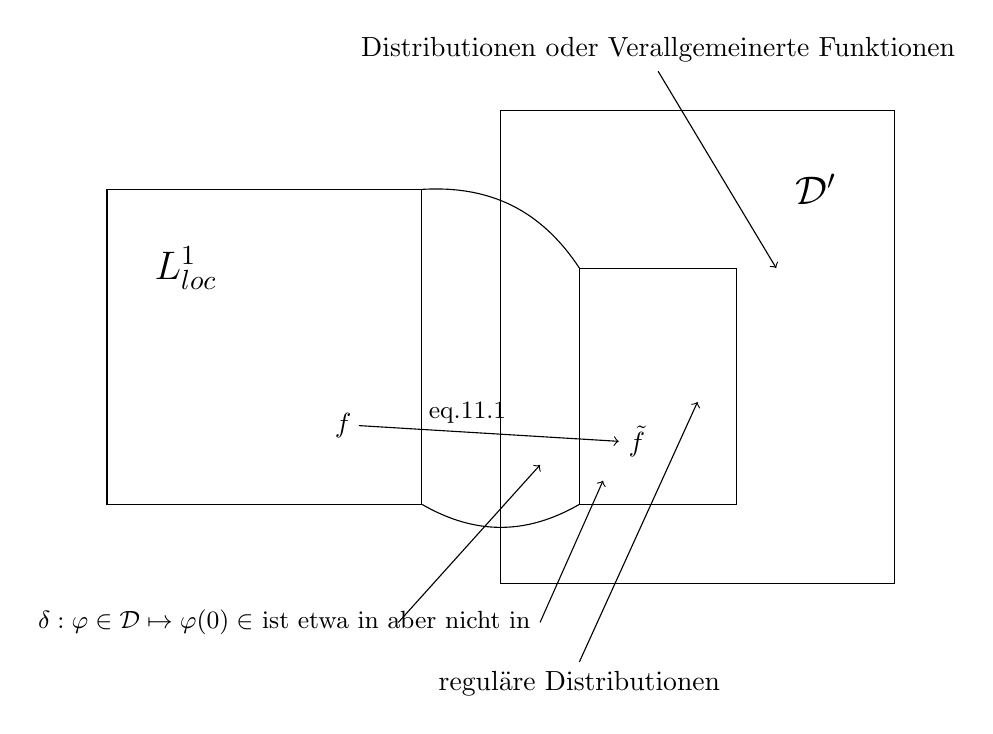
\begin{tikzpicture}
        \draw (0,0) rectangle (4,4);
        \draw (1,3) node[] {\Large $L^1_{loc}$};
        \draw (3,1) node[] {$f$};
        \draw (5,-1) rectangle (10,5);
        \draw (6,0) rectangle (8,3);
        \draw (4,4) to[bend left] (6,3);
        \draw (4,0) to[bend right] (6,0);
        \draw[->] (3.2,1) -- node[above]{\small \eqref{eq.11.1} \ \ \ \ \ } (6.5,0.8) node[right] {$\tilde f$};
        \draw (9,4) node[] {\Large $\D'$};
        \draw[<-] (7.5,1.3) -- (6,-2) node[below]{reguläre Distributionen};
        \draw[<-] (8.5,3) -- (7,5.5) node[above]{\mim{Distributionen} oder Verallgemeinerte Funktionen};
        \draw (-1,-1.5) node[right] {\small $\delta:\varphi \in \D \mapsto \varphi(0) \in \R$ ist etwa in  aber nicht in};
        \draw[<-] (6.3,0.3) -- (5.5,-1.5);
        \draw[<-] (5.5,0.5) -- (3.7,-1.5);
    \end{tikzpicture}
\end{center}

Nun zu den Abbleitungen, sein zunächst $d=1$ und $f \in C^1 \subset L^1_{loc}$, dann gilt für alle $\varphi \in \D$ wobei $[-a,a] \supset supp(\varphi)$:

\[\underbrace{\int_{\R^1} f'(x) \varphi(x) dx}_{f'(\varphi)} = \int_{-a}^a f(x) \phi(x) dx = \underbrace{f(x)\varphi(x)|_{-a}^{a}}_{=0} - \int_{-a}^a f(x) \varphi'(x) dx = -\int_{\R^1} f(x) \varphi'(x) dx = -\tilde f(\varphi')\]

$\Rightarrow$ Für $f \in C^1 \subset L^1_{loc}$ gilt $\tilde f'(\varphi) = - \tilde f(\varphi'), \varphi \in \D$. Wir nehmen dies als Ansatz und setzen:

\begin{equation}\label{eq.11.2}
    F'(\varphi):=-F(\varphi'), \varphi \in \D
\end{equation}

für alle $F\in \D$, genannt Distributionen Abbleitung.

Beispiel:

\begin{center}
    \begin{tikzpicture}
        \draw (-0.4,0) node[left] {$f(x) = \abs{x}$};
        \draw (-0.2,0) -- (4.2,0);
        \draw[thick] (0,2) -- (2,0) -- (4,2);
        \draw (2,-0.1) -- (2,2.3);
    \end{tikzpicture}
\end{center}
Und $F:=\tilde f$ also:

\[F'(\varphi) = -F(\varphi) = - \int_{-a}^a \abs{x} \varphi'(x) dx = - \int_{-a}^0 -x \varphi'(x) dx - \int_0^a x \varphi'(x) dx \]

\[= \int_{-a}^0 x \varphi'(x) dx - \int_0^a x \varphi'(x) dx = \underbrace{x \varphi(x)|_{-a}^0}_{0} - \int_{-a}^0 1 \varphi(x) dx - \underbrace{x \varphi(x)|_0^a}_{0} + \int_0^a 1 \varphi(x) dx\]

\[= \int_{-a}^a sing(x) \varphi(x) dx = \tilde{sign}(\varphi)\]

\begin{center}
    \begin{tikzpicture}
        \draw (-0.4,0) node[left] {$sign(x)=$};
        \draw (-0.2,0) -- (4.2,0);
        \draw (2,-1.3) -- (2,1.3);
        \draw[thick] (2,1) node[left]{\small $1$} -- (4,1);
        \draw[thick] (0,-1) -- (2,-1) node[right]{\small $-1$};
    \end{tikzpicture}
\end{center}

Also insgesamt $F'=\tilde{sign}$